\section{\heiti 引言}

随着信息技术的飞速发展,“数字法院”的建设已成为全球司法领域现代化的重要趋势,对司法审判智能化解决方案的需求日益迫切,尤其在刑事案件审判领域,其核心目标在于提升司法判决的准确性、一致性与效率~\cite{aletras2016predicting}。在这一背景下,法律判决预测(Legal Judgment Prediction, LJP)作为法律人工智能领域的一项基础性、关键性研究任务,受到了学术界与实务界的广泛关注。LJP旨在通过分析案件的事实描述,自动预测法院可能的判决结果,从而辅助法官及其他法律从业者,提高案件处理效率.

LJP技术早期研究主要依赖于人工构建的规则系统和传统的统计机器学习方法~\cite{katz2017general,keown1980mathematical}, 例如支持向量机支持向量机(Support Vector  Machine , SVM)~\cite{boella2011using,kim2015legal}。Sulea~\cite{sulea2017exploring}构建了一种结合多个SVM分类器输出的平均概率集成系统,模型以案情事实描述和时间跨度信息作为输入,能够输出判决结果、法律范围、估算判决日期等信息。Katz[21]使用随机森林,从案情描述中提取有效特征对美国最高法院的判决结果进行预测。但这些方法尚不能挖掘深层的文本特征,且因人工设计的特性,需要大量的人力成本,无法深入应用到其他领域。

然而,传统的自然语言处理和机器学习模型在应用于LJP任务时,往往难以充分捕捉法律文本中复杂的逻辑依赖关系,也难以清晰地呈现法律推理过程~\cite{lin2012exploiting,liu2004case}。
此外,许多早期的深度学习LJP模型如同“黑箱”般运作,其决策过程缺乏透明度和可解释性。不可解释性构成了模型在司法实践中推广应用的主要障碍\cite{ling2017program,ma2021law}。法官难以干预模型的审判逻辑或理解其预测依据,削弱了模型的实用价值。缺乏可解释性还可能引发伦理问题。尤其是模型从历史数据中学习到潜在的偏见,可能导致不公正或不一致的判决结果~\cite{luo2017learning,lv2022improving}。
大型语言模型(LLM)虽因其卓越的语言理解能力而备受期待~\cite{jiang2023legal},但在法律领域的直接应用暴露出若干固有缺陷。
一个核心问题是LLM倾向于产生“幻觉”(Hallucinations)~\cite{lewis2020retrieval},即生成与客观事实或用户输入不符的内容 。在法律语境下,这可能表现为援引虚假的判例、引言或内部引证,其后果不堪设想。研究表明,在处理特定法律查询时,LLM的幻觉率可能高达69\%至88\%~\cite{Dahl_2024},这种现象往往源于模型在缺乏可验证法律依据的情况下尝试进行推理或生成信息。

为了解决传统方法在可解释性和处理复杂法律逻辑方面存在不足,而直接应用通用大型语言模型则面临幻觉、缺乏法律知识基础和专业推理能力等问题。因此,本研究提出法律指导的类案融合判决方法,通过提取判决核心要素——犯罪核心要素与证据核心要素,为判决减少干扰因素,提供准确和核心的信息。通过引入法律条文数据库, 为模型提供明确的权威的法律依据,弥补其法律知识的不足,并减少判决“幻觉”现象。 此外,本研究还引入相似案例,旨在为LLM提供司法实践层面的参考,使其理解法律条文在具体情境下的应用方式,学习裁判经验。最后LLM作为核心推理引擎,对这些多源异构信息进行综合分析与推理,综合考量法律原则、司法解释及类案判例的指导作用,输出结构化的判决结果。本研究的方法无需对整个大模型进行重新训练,将复杂的LJP任务分解多个子任务,使得整个推理过程更为透明和模块化。与一些端到端的黑箱模型相比,这种设计不仅有助于提升整体预测的鲁棒性,也为理解和调试模型行为提供了便利。

\begin{figure*}[htbp]
	\centering
	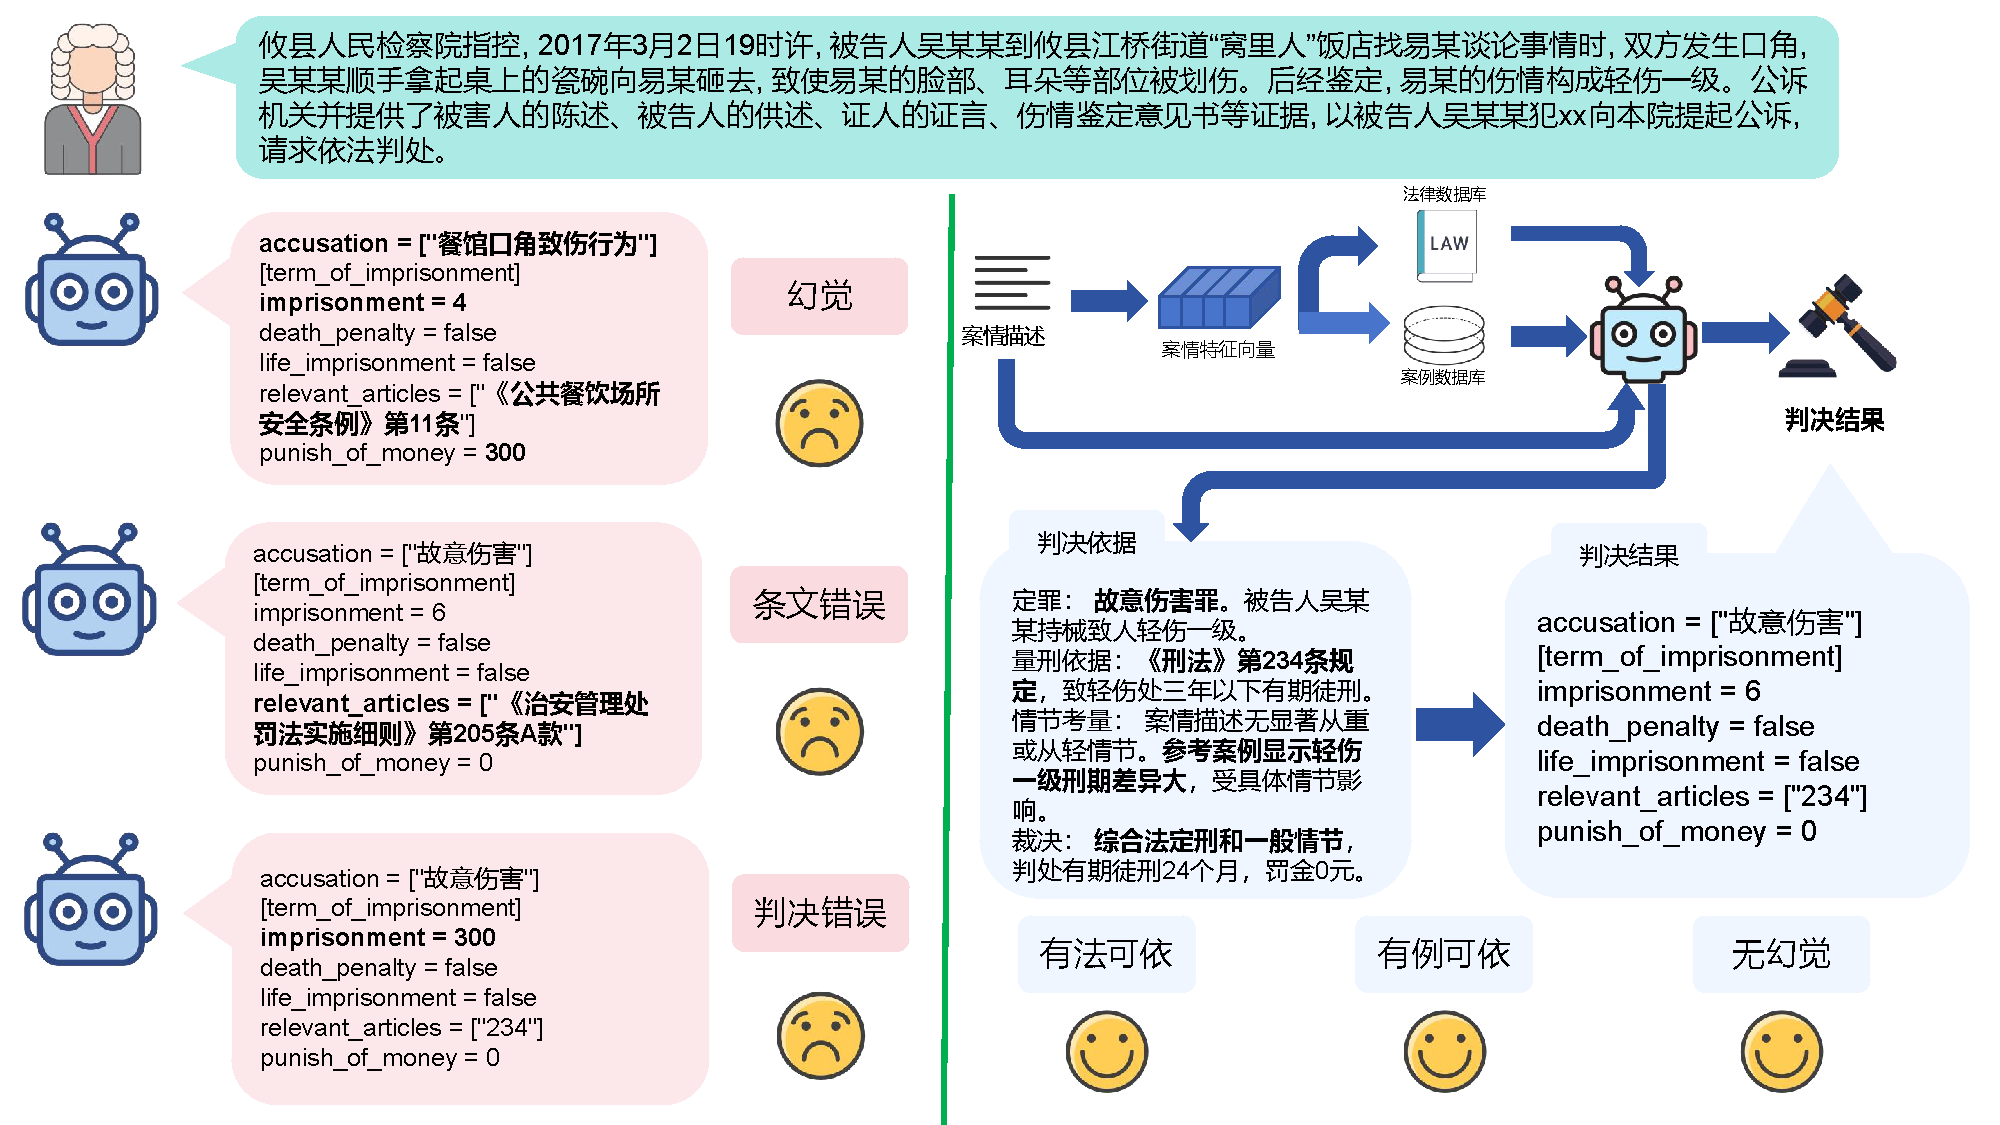
\includegraphics[width=1\textwidth]{fig/motivation.pdf}
	\caption{动机}
	\label{fig:motivation}
\end{figure*}